% =====================================================================
%  FarmaVita · Informe técnico de infraestructura segura
%  Estilo editorial "Sultana del Lago Editores" adaptado a FarmaVita
%  Compilar: pdflatex informe_farmavita.tex  (dos pasadas para el índice)
% =====================================================================
\documentclass[11pt,a4paper,oneside]{report}

% ---------------------------------------------------------------------
%  Idioma y codificación
% ---------------------------------------------------------------------
\usepackage[utf8]{inputenc}
\usepackage[T1]{fontenc}
\IfFileExists{spanish.ldf}{%
  \usepackage[spanish,es-noshorthands,es-tabla]{babel}%
}{%
  % Respaldo si la distribución no incluye babel-spanish
  \usepackage[english]{babel}%
  \addto\captionsenglish{%
    \renewcommand{\contentsname}{Índice general}%
    \renewcommand{\listfigurename}{Índice de figuras}%
    \renewcommand{\listtablename}{Índice de tablas}%
    \renewcommand{\figurename}{Figura}%
    \renewcommand{\tablename}{Tabla}%
    \renewcommand{\chaptername}{Capítulo}%
    \renewcommand{\appendixname}{Anexo}%
    \renewcommand{\bibname}{Referencias}%
  }%
}

% ---------------------------------------------------------------------
%  Tipografía editorial: Palatino (texto) + Helvética (titulares)
% ---------------------------------------------------------------------
\usepackage{mathpazo}
\usepackage[scaled=0.92]{helvet}
\usepackage{microtype}
\linespread{1.08}

% ---------------------------------------------------------------------
%  Paquetes
% ---------------------------------------------------------------------
\usepackage[top=2.6cm,bottom=2.6cm,left=2.8cm,right=2.4cm,headheight=15pt]{geometry}
\usepackage[table]{xcolor}
\usepackage{graphicx}
\usepackage{tikz}
\usetikzlibrary{positioning,arrows.meta,shapes.geometric,shapes.misc,fit,backgrounds,calc,shadows}
\usepackage{booktabs}
\usepackage{tabularx}
\usepackage{longtable}
\usepackage{array}
\usepackage{multirow}
\usepackage{enumitem}
\usepackage{fancyhdr}
\usepackage{titlesec}
\usepackage{listings}
\usepackage[most]{tcolorbox}
\usepackage{siunitx}
\sisetup{output-decimal-marker={,},group-separator={.},group-minimum-digits=4,per-mode=symbol}
\usepackage{amsmath,amssymb}
\DeclareSIUnit\voltampere{VA}
\usepackage[hidelinks]{hyperref}

% ---------------------------------------------------------------------
%  Identidad cromática FarmaVita / Sultana del Lago
% ---------------------------------------------------------------------
\definecolor{fvVerde}{HTML}{0F766E}
\definecolor{fvVerdeOsc}{HTML}{134E4A}
\definecolor{fvVerdeClaro}{HTML}{CCFBF1}
\definecolor{fvTinta}{HTML}{0F172A}
\definecolor{fvGris}{HTML}{64748B}
\definecolor{fvArena}{HTML}{F5F1E8}
\definecolor{fvOro}{HTML}{B8860B}
\definecolor{fvRojo}{HTML}{B91C1C}
\definecolor{fvAzul}{HTML}{1D4ED8}
\definecolor{fvAmbar}{HTML}{B45309}

\hypersetup{pdftitle={FarmaVita - Informe técnico de infraestructura segura},
            pdfauthor={Sultana del Lago Editores},
            pdfsubject={Seguridad Informática - URU}}

% ---------------------------------------------------------------------
%  Títulos de capítulo y sección (estilo editorial)
% ---------------------------------------------------------------------
\titleformat{\chapter}[display]
  {\sffamily\bfseries\color{fvTinta}}
  {\color{fvOro}\large\MakeUppercase{\chaptertitlename}~\thechapter\hspace{0.6em}\textcolor{fvVerde}{\rule[0.3ex]{0.55\textwidth}{0.6pt}}}
  {4pt}
  {\Huge}
  [\vspace{2pt}{\color{fvVerde}\titlerule[1.2pt]}]
\titlespacing*{\chapter}{0pt}{-10pt}{24pt}

\titleformat{\section}
  {\sffamily\Large\bfseries\color{fvVerdeOsc}}{\textcolor{fvOro}{\thesection}}{0.8em}{}
\titleformat{\subsection}
  {\sffamily\large\bfseries\color{fvTinta}}{\textcolor{fvVerde}{\thesubsection}}{0.7em}{}
\titleformat{\subsubsection}
  {\sffamily\normalsize\bfseries\color{fvGris}}{}{0em}{}

% ---------------------------------------------------------------------
%  Encabezado y pie
% ---------------------------------------------------------------------
\pagestyle{fancy}
\fancyhf{}
\renewcommand{\headrulewidth}{0.4pt}
\renewcommand{\headrule}{\hbox to\headwidth{\color{fvVerde}\leaders\hrule height \headrulewidth\hfill}}
\fancyhead[L]{\sffamily\footnotesize\color{fvGris}FarmaVita · Infraestructura segura}
\fancyhead[R]{\sffamily\footnotesize\color{fvGris}\leftmark}
\fancyfoot[L]{\sffamily\scriptsize\color{fvOro}SULTANA DEL LAGO EDITORES}
\fancyfoot[R]{\sffamily\footnotesize\bfseries\color{fvVerde}\thepage}
\fancypagestyle{plain}{%
  \fancyhf{}\renewcommand{\headrulewidth}{0pt}%
  \fancyfoot[L]{\sffamily\scriptsize\color{fvOro}SULTANA DEL LAGO EDITORES}%
  \fancyfoot[R]{\sffamily\footnotesize\bfseries\color{fvVerde}\thepage}}
\renewcommand{\chaptermark}[1]{\markboth{#1}{}}

% ---------------------------------------------------------------------
%  Cajas editoriales
% ---------------------------------------------------------------------
\newtcolorbox{destacado}[1][]{enhanced,breakable,colback=fvArena,colframe=fvOro,
  boxrule=0pt,leftrule=3pt,arc=0pt,left=10pt,right=10pt,top=6pt,bottom=6pt,
  fonttitle=\sffamily\bfseries\color{fvOro},coltitle=fvOro,colbacktitle=fvArena,
  title={#1},attach title to upper={\par\smallskip}}
\newtcolorbox{critico}[1][]{enhanced,breakable,colback=red!3,colframe=fvRojo,
  boxrule=0pt,leftrule=3pt,arc=0pt,left=10pt,right=10pt,top=6pt,bottom=6pt,
  fonttitle=\sffamily\bfseries,coltitle=fvRojo,colbacktitle=red!3,
  title={#1},attach title to upper={\par\smallskip}}
\newtcolorbox{tecnico}[1][]{enhanced,breakable,colback=fvVerdeClaro!40,colframe=fvVerde,
  boxrule=0pt,leftrule=3pt,arc=0pt,left=10pt,right=10pt,top=6pt,bottom=6pt,
  fonttitle=\sffamily\bfseries,coltitle=fvVerdeOsc,colbacktitle=fvVerdeClaro!40,
  title={#1},attach title to upper={\par\smallskip}}

% ---------------------------------------------------------------------
%  Listados de código
% ---------------------------------------------------------------------
\lstdefinelanguage{nft}{
  morekeywords={table,chain,type,hook,priority,policy,accept,drop,counter,define,
    masquerade,flush,ruleset,ip,saddr,daddr,ct,state,iif,oifname,tcp,dport,icmp,comment,filter,nat,inet},
  sensitive=true, morecomment=[l]{\#}, morestring=[b]"}
\lstset{
  basicstyle=\ttfamily\footnotesize,
  keywordstyle=\color{fvVerde}\bfseries,
  commentstyle=\color{fvGris}\itshape,
  stringstyle=\color{fvAmbar},
  backgroundcolor=\color{fvArena},
  frame=leftline, framerule=2pt, rulecolor=\color{fvVerde},
  xleftmargin=8pt, framexleftmargin=6pt,
  breaklines=true, columns=fullflexible, keepspaces=true,
  showstringspaces=false, numbers=none,
  aboveskip=8pt, belowskip=8pt,
  literate={á}{{\'a}}1 {é}{{\'e}}1 {í}{{\'i}}1 {ó}{{\'o}}1 {ú}{{\'u}}1 {ñ}{{\~n}}1
           {Á}{{\'A}}1 {É}{{\'E}}1 {Í}{{\'I}}1 {Ó}{{\'O}}1 {Ú}{{\'U}}1 {Ñ}{{\~N}}1
}

% ---------------------------------------------------------------------
%  Utilidades
% ---------------------------------------------------------------------
\newcolumntype{L}[1]{>{\raggedright\arraybackslash}p{#1}}
\newcolumntype{C}[1]{>{\centering\arraybackslash}p{#1}}
\newcommand{\permitir}{\textcolor{green!45!black}{\textbf{PERMITIR}}}
\newcommand{\denegar}{\textcolor{fvRojo}{\textbf{DENEGAR}}}
\newcommand{\cod}[1]{\texttt{\small #1}}
\renewcommand{\arraystretch}{1.25}
\setlist{itemsep=2pt,topsep=4pt}

% =====================================================================
\begin{document}
% =====================================================================

% ------------------------------- PORTADA -----------------------------
\begin{titlepage}
\begin{tikzpicture}[remember picture,overlay]
  \fill[fvVerdeOsc] (current page.north west) rectangle ([yshift=-11cm]current page.north east);
  \fill[fvOro] ([yshift=-11cm]current page.north west) rectangle ([yshift=-11.25cm]current page.north east);
  \fill[fvArena] ([yshift=-11.25cm]current page.north west) rectangle (current page.south east);
  % Cruz farmacéutica estilizada
  \begin{scope}[shift={([xshift=-4cm,yshift=-5.6cm]current page.north east)},opacity=0.18]
    \fill[white] (-0.9,-2.7) rectangle (0.9,2.7);
    \fill[white] (-2.7,-0.9) rectangle (2.7,0.9);
  \end{scope}
  \node[anchor=north west,text=white,font=\sffamily\small\bfseries,inner sep=0]
    at ([xshift=2.8cm,yshift=-2.2cm]current page.north west)
    {SULTANA DEL LAGO EDITORES \textcolor{fvOro}{\textbullet} COLECCIÓN SEGURIDAD INFORMÁTICA};
  \node[anchor=north west,text=white,font=\sffamily\fontsize{44}{48}\selectfont\bfseries,inner sep=0]
    at ([xshift=2.8cm,yshift=-3.6cm]current page.north west) {FarmaVita};
  \node[anchor=north west,text=fvVerdeClaro,font=\sffamily\LARGE,inner sep=0,text width=13cm]
    at ([xshift=2.8cm,yshift=-5.6cm]current page.north west)
    {Infraestructura empresarial contenerizada para distribución y laboratorio farmacéutico};
  \node[anchor=north west,text=white,font=\large\itshape,inner sep=0,text width=13cm]
    at ([xshift=2.8cm,yshift=-8.1cm]current page.north west)
    {Defensa en profundidad, microsegmentación Zero Trust, control de acceso basado en roles y continuidad operativa de 72 horas};
\end{tikzpicture}

\vspace*{11.2cm}
\begin{flushleft}
\hspace*{0.4cm}\begin{minipage}{0.86\textwidth}
\sffamily
{\color{fvOro}\rule{2.5cm}{2pt}}\par\vspace{0.6cm}
{\Large\bfseries\color{fvTinta} Informe técnico de arquitectura}\par\vspace{0.25cm}
{\large\color{fvGris} proyectoFarmaVita\_SEG.INF-URU}\par\vspace{1.2cm}

\begin{tabular}{@{}L{4.2cm}L{9cm}@{}}
\textcolor{fvGris}{Asignatura} & Seguridad Informática \\
\textcolor{fvGris}{Institución} & Universidad Rafael Urdaneta (URU) \\
\textcolor{fvGris}{Ámbito} & Distribuidora y laboratorio farmacéutico \\
\textcolor{fvGris}{Componentes} & Docker Compose · nftables · Nginx · OpenLDAP · NestJS · PostgreSQL · React · Rust \\
\textcolor{fvGris}{Versión} & 1.0 · noviembre de 2026 \\
\end{tabular}
\end{minipage}
\end{flushleft}

\vfill
\begin{center}
\sffamily\scriptsize\color{fvGris}
Maracaibo, Venezuela \textbullet{} Edición FarmaVita de Sultana del Lago Editores \textbullet{} Documento de uso académico
\end{center}
\end{titlepage}

% ------------------------------- ÍNDICES -----------------------------
\pagenumbering{roman}
\tableofcontents
\listoffigures
\listoftables
\clearpage
\pagenumbering{arabic}

% =====================================================================
\chapter*{Resumen ejecutivo}
\addcontentsline{toc}{chapter}{Resumen ejecutivo}
\markboth{Resumen ejecutivo}{}
% =====================================================================

FarmaVita es la infraestructura tecnológica de una distribuidora y laboratorio farmacéutico
que almacena, controla y dispensa medicamentos, incluidos productos biológicos que exigen
\emph{cadena de frío} (\SIrange{2}{8}{\celsius}). La solución se entrega como un conjunto de
servicios contenerizados desplegables con un único comando
(\cod{docker compose up -d --build}) y se apoya en tres pilares:

\begin{enumerate}[label=\textbf{\arabic*.},leftmargin=*]
  \item \textbf{Prevención de ransomware.} La base de datos PostgreSQL reside en una red
  exclusiva (VLAN~40, \cod{10.10.40.0/24}) que \emph{ninguna} estación de trabajo puede alcanzar.
  El firewall perimetral \cod{fw-01} aplica una política \emph{forward} de denegación por
  defecto: sólo la red de aplicaciones puede abrir conexiones TCP/5432 hacia el servidor de
  datos. Un equipo de oficina comprometido por un \emph{ransomware} no puede cifrar,
  exfiltrar ni siquiera descubrir (ICMP bloqueado) el activo de información más crítico.

  \item \textbf{Trazabilidad farmacéutica.} Ningún medicamento puede venderse o dispensarse
  si no cuenta con al menos un lote evaluado y \textsc{aprobado} por Laboratorio. La regla
  se aplica en el servidor (NestJS), no en la interfaz, y se reverifica dentro de una
  transacción con bloqueo pesimista (\cod{SELECT \dots{} FOR UPDATE}) que, además, impide
  saldos de inventario negativos ante ventas concurrentes. Cada evaluación registra el
  analista (identidad LDAP), la temperatura medida y la fecha; una excursión térmica
  impide aprobar el lote.

  \item \textbf{Continuidad operativa.} La arquitectura eléctrica combina un SAI/UPS de
  doble conversión en línea (\SI{20}{\kilo\voltampere}) con un grupo electrógeno diésel de
  \SI{80}{\kilo\voltampere} y conmutador de transferencia automática (ATS), con un tanque
  dimensionado para \SI{72}{\hour} de autonomía a plena carga y reserva superior al
  \SI{40}{\percent}, preservando la cadena de frío ante cortes prolongados.
\end{enumerate}

\begin{destacado}[Principios de diseño]
\textbf{Defensa en profundidad}: perímetro (nftables) $\rightarrow$ DMZ con proxy inverso
(Nginx) $\rightarrow$ autenticación centralizada (OpenLDAP) $\rightarrow$ autorización
por roles (JWT + \cod{RolesGuard}) $\rightarrow$ validación de negocio y transacciones
$\rightarrow$ auditoría en base de datos.
\textbf{Zero Trust interno}: siete segmentos aislados; la confianza nunca se infiere de la
ubicación en la red, cada petición porta un token firmado y cada flujo entre segmentos
se autoriza explícitamente.
\end{destacado}

% =====================================================================
\chapter{Topología lógica}
% =====================================================================

\section{Visión general}

La red se compone de siete subredes Docker de tipo \emph{bridge}, cada una equivalente a
una VLAN de la infraestructura física. El contenedor \cod{fw-01} está conectado a las
siete y actúa como único punto de interconexión: posee la dirección \cod{.254} en cada
segmento, tiene habilitado \cod{net.ipv4.ip\_forward=1} y filtra con nftables. Las
estaciones de oficina reemplazan su ruta por defecto para apuntar a \cod{fw-01} y
\textbf{no publican puertos} hacia el anfitrión.

\begin{figure}[htbp]
\centering
\begin{tikzpicture}[
  font=\sffamily\scriptsize,
  red/.style={draw=#1,fill=#1!8,rounded corners=4pt,thick,minimum width=3.6cm,minimum height=2.1cm,align=center,text width=3.4cm},
  srv/.style={draw=fvTinta!60,fill=white,rounded corners=2pt,inner sep=3pt,font=\sffamily\tiny,align=center},
  enlace/.style={-,thick,draw=fvGris},
  ok/.style={-{Stealth[length=2.2mm]},thick,draw=green!45!black},
  no/.style={-{Stealth[length=2.2mm]},thick,draw=fvRojo,dashed},
  node distance=1.2cm
]
  % Firewall central
  \node[draw=fvTinta,fill=fvTinta,text=white,rounded corners=6pt,minimum width=3.2cm,
        minimum height=1.3cm,align=center,font=\sffamily\small\bfseries,drop shadow] (fw)
        {fw-01\\[-1pt]{\tiny\mdseries nftables · forward DROP · NAT}};

  % Servidores (fila superior)
  \node[red=fvAmbar, above left=1.6cm and 1.3cm of fw] (dmz)
     {\textbf{red\_dmz · VLAN 20}\\10.10.20.0/24\\[3pt]
      \tikz\node[srv]{Nginx proxy inverso\\10.10.20.10\\intranet.farmaceutica.local};};
  \node[red=fvVerde, above=1.6cm of fw] (apps)
     {\textbf{red\_apps · VLAN 30}\\10.10.30.0/24\\[3pt]
      \tikz\node[srv]{NestJS API · 10.10.30.20\\OpenLDAP · 10.10.30.30};};
  \node[red=fvAzul, above right=1.6cm and 1.3cm of fw] (datos)
     {\textbf{red\_datos · VLAN 40}\\10.10.40.0/24\\[3pt]
      \tikz\node[srv]{PostgreSQL farma\_db\\10.10.40.10};};

  % Oficinas (fila inferior)
  \node[red=fvGris, below left=1.7cm and 2.3cm of fw, minimum width=2.9cm,text width=2.7cm] (alm)
     {\textbf{VLAN 210 Almacén}\\10.10.210.0/24\\[2pt]\tikz\node[srv]{pc\_almacen\_01\\TUI Rust};};
  \node[red=fvGris, right=0.35cm of alm, minimum width=2.9cm,text width=2.7cm] (ven)
     {\textbf{VLAN 220 Ventas}\\10.10.220.0/24\\[2pt]\tikz\node[srv]{pc\_ventas\_01};};
  \node[red=fvGris, right=0.35cm of ven, minimum width=2.9cm,text width=2.7cm] (adm)
     {\textbf{VLAN 230 Admin.}\\10.10.230.0/24\\[2pt]\tikz\node[srv]{pc\_admin\_01};};
  \node[red=fvGris, right=0.35cm of adm, minimum width=2.9cm,text width=2.7cm] (lab)
     {\textbf{VLAN 240 Laboratorio}\\10.10.240.0/24\\[2pt]\tikz\node[srv]{pc\_laboratorio\_01};};

  % Enlaces físicos al firewall
  \foreach \n/\ip in {dmz/.20.254, apps/.30.254, datos/.40.254} {
    \draw[enlace] (\n.south) -- (fw) node[pos=0.45,fill=white,inner sep=1pt,font=\sffamily\tiny]{\ip};
  }
  \foreach \n/\ip in {alm/.210.254, ven/.220.254, adm/.230.254, lab/.240.254} {
    \draw[enlace] (\n.north) -- (fw) node[pos=0.5,fill=white,inner sep=1pt,font=\sffamily\tiny]{\ip};
  }

  % Flujos lógicos
  \draw[ok] (dmz.east) to[bend left=12] node[above,font=\sffamily\tiny,text=green!45!black]{TCP/3000} (apps.west);
  \draw[ok] (apps.east) to[bend left=12] node[above,font=\sffamily\tiny,text=green!45!black]{TCP/5432} (datos.west);
  \draw[no] (lab.east) .. controls +(2.2,0.4) and +(0.6,-2.6) .. (datos.south east)
     node[pos=0.55,right,font=\sffamily\tiny\bfseries,text=fvRojo,align=left]{Oficinas $\rightarrow$ Datos\\BLOQUEADO};
\end{tikzpicture}
\caption{Topología lógica de FarmaVita: siete segmentos interconectados exclusivamente por \cod{fw-01}.}
\label{fig:topologia}
\end{figure}

\section{Tabla de direccionamiento}

\begin{table}[htbp]
\centering\small
\caption{Direccionamiento de las siete VLAN/subredes y sus hosts.}
\label{tab:direccionamiento}
\rowcolors{2}{fvArena}{white}
\begin{tabularx}{\textwidth}{@{}l l l l X@{}}
\toprule
\rowcolor{fvVerdeOsc}
\textcolor{white}{\textbf{VLAN}} & \textcolor{white}{\textbf{Red Docker}} & \textcolor{white}{\textbf{Subred}} &
\textcolor{white}{\textbf{Gateway}} & \textcolor{white}{\textbf{Hosts / función}} \\
\midrule
20  & \cod{red\_dmz}             & 10.10.20.0/24  & 10.10.20.254  & \cod{farma\_proxy} 10.10.20.10 (Nginx + React) \\
30  & \cod{red\_apps}            & 10.10.30.0/24  & 10.10.30.254  & \cod{farma\_backend} .20 (NestJS) · \cod{farma\_ldap} .30 \\
40  & \cod{red\_datos}           & 10.10.40.0/24  & 10.10.40.254  & \cod{farma\_db} 10.10.40.10 (PostgreSQL 16) \\
210 & \cod{vlan210\_almacen}     & 10.10.210.0/24 & 10.10.210.254 & \cod{pc\_almacen\_01} .10 (cliente TUI Rust) \\
220 & \cod{vlan220\_ventas}      & 10.10.220.0/24 & 10.10.220.254 & \cod{pc\_ventas\_01} .10 \\
230 & \cod{vlan230\_admin}       & 10.10.230.0/24 & 10.10.230.254 & \cod{pc\_admin\_01} .10 \\
240 & \cod{vlan240\_laboratorio} & 10.10.240.0/24 & 10.10.240.254 & \cod{pc\_laboratorio\_01} .10 \\
\bottomrule
\end{tabularx}
\end{table}

\section{Enrutamiento}

\begin{itemize}
  \item \textbf{Estaciones de oficina}: al iniciar ejecutan \cod{ip route replace default via
  10.10.2x0.254}, de modo que todo su tráfico atraviesa el firewall. Disponen de la
  capacidad \cod{NET\_ADMIN} únicamente para fijar esta ruta.
  \item \textbf{Proxy de la DMZ}: ruta estática \cod{10.10.30.0/24 via 10.10.20.254} para
  alcanzar la API a través de \cod{fw-01}.
  \item \textbf{API NestJS}: ruta estática \cod{10.10.40.0/24 via 10.10.30.254}; OpenLDAP
  comparte su segmento y se alcanza de forma directa.
  \item \textbf{Base de datos}: no necesita rutas adicionales; las conexiones le llegan
  enmascaradas con la IP \cod{10.10.40.254}, por lo que la respuesta retorna siempre por
  el firewall (enrutamiento simétrico).
\end{itemize}

% =====================================================================
\chapter{Gestión de identidades}
% =====================================================================

\section{Directorio corporativo OpenLDAP}

El servicio \cod{farma\_ldap} (imagen \cod{osixia/openldap}) publica el árbol
\cod{dc=farmaceutica,dc=local}. Durante el primer arranque se carga automáticamente el
archivo LDIF \cod{01-farmaceutica.ldif} (carpeta \cod{ldap/bootstrap/}), que crea las unidades organizativas
\cod{ou=usuarios} y \cod{ou=grupos}, las cuentas y los grupos de rol (\cod{groupOfNames}).

\begin{table}[htbp]
\centering\small
\caption{Identidades iniciales del directorio.}
\label{tab:usuarios}
\rowcolors{2}{fvArena}{white}
\begin{tabular}{@{}l l l l@{}}
\toprule
\rowcolor{fvVerdeOsc}
\textcolor{white}{\textbf{uid}} & \textcolor{white}{\textbf{Contraseña inicial}} &
\textcolor{white}{\textbf{VLAN}} & \textcolor{white}{\textbf{Grupo / rol}} \\
\midrule
\cod{almacenista1}   & \cod{password\_almacen\_123} & 210 & \cod{cn=almacen} \\
\cod{farmaceutico1}  & \cod{password\_ventas\_123}  & 220 & \cod{cn=ventas} \\
\cod{laboratorista1} & \cod{password\_lab\_123}     & 240 & \cod{cn=laboratorio} \\
\cod{admin1}         & \cod{password\_admin\_123}   & 230 & \cod{cn=admin} (supervisión) \\
\bottomrule
\end{tabular}
\end{table}

\section{Flujo técnico OpenLDAP $\rightarrow$ JWT $\rightarrow$ RBAC}

\begin{figure}[htbp]
\centering
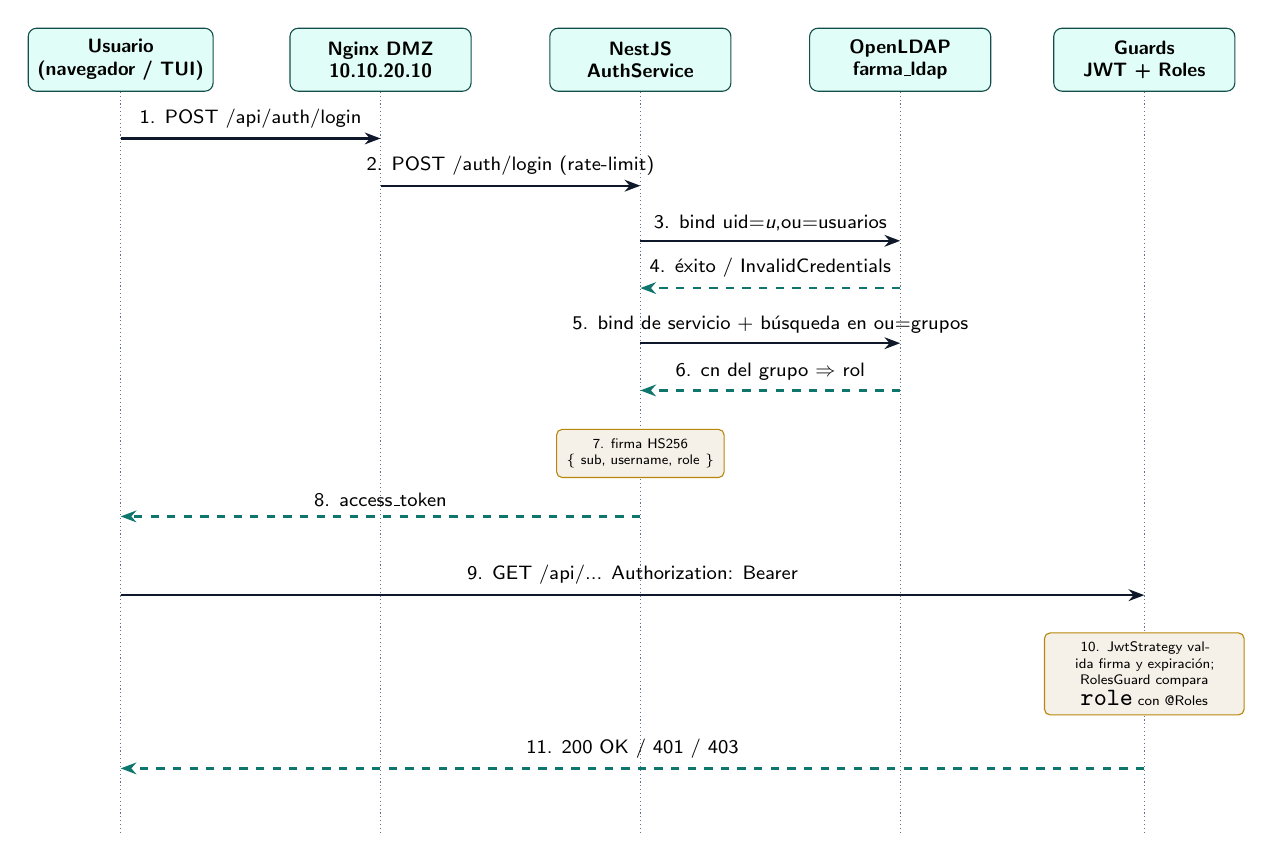
\begin{tikzpicture}[
  font=\sffamily\scriptsize,
  actor/.style={draw=fvVerdeOsc,fill=fvVerdeClaro!60,rounded corners=3pt,minimum width=2.3cm,minimum height=0.8cm,align=center,font=\sffamily\scriptsize\bfseries},
  msg/.style={-{Stealth[length=2mm]},thick,draw=fvTinta},
  ret/.style={-{Stealth[length=2mm]},thick,dashed,draw=fvVerde},
]
  \node[actor] (u) at (0,0) {Usuario\\(navegador / TUI)};
  \node[actor] (n) at (3.3,0) {Nginx DMZ\\10.10.20.10};
  \node[actor] (a) at (6.6,0) {NestJS\\AuthService};
  \node[actor] (l) at (9.9,0) {OpenLDAP\\farma\_ldap};
  \node[actor] (r) at (13.0,0) {Guards\\JWT + Roles};
  \foreach \x in {u,n,a,l,r} \draw[fvGris,densely dotted] (\x.south) -- ++(0,-9.4);

  \draw[msg] (0,-1.0) -- node[above]{1. POST /api/auth/login} (3.3,-1.0);
  \draw[msg] (3.3,-1.6) -- node[above]{2. POST /auth/login (rate-limit)} (6.6,-1.6);
  \draw[msg] (6.6,-2.3) -- node[above,align=center]{3. bind uid=\textit{u},ou=usuarios} (9.9,-2.3);
  \draw[ret] (9.9,-2.9) -- node[above]{4. éxito / InvalidCredentials} (6.6,-2.9);
  \draw[msg] (6.6,-3.6) -- node[above,align=center]{5. bind de servicio + búsqueda en ou=grupos} (9.9,-3.6);
  \draw[ret] (9.9,-4.2) -- node[above]{6. cn del grupo $\Rightarrow$ rol} (6.6,-4.2);
  \node[draw=fvOro,fill=fvArena,rounded corners=2pt,align=center,font=\sffamily\tiny] at (6.6,-5.0)
     {7. firma HS256\\\{ sub, username, role \}};
  \draw[ret] (6.6,-5.8) -- node[above]{8. access\_token} (0,-5.8);
  \draw[msg] (0,-6.8) -- node[above]{9. GET /api/... Authorization: Bearer} (13.0,-6.8);
  \node[draw=fvOro,fill=fvArena,rounded corners=2pt,align=center,font=\sffamily\tiny,text width=2.3cm] at (13.0,-7.8)
     {10. JwtStrategy valida firma y expiración; RolesGuard compara \cod{role} con @Roles};
  \draw[ret] (13.0,-9.0) -- node[above]{11. 200 OK / 401 / 403} (0,-9.0);
\end{tikzpicture}
\caption{Secuencia de autenticación (LDAP bind) y autorización (JWT + RBAC).}
\label{fig:flujo-auth}
\end{figure}

\subsection{Autenticación por bind directo}
El \cod{LdapService} construye el DN \cod{uid=<usuario>,ou=usuarios,dc=farmaceutica,dc=local}
y ejecuta un \emph{bind} con la contraseña recibida: el servidor LDAP es quien valida la
credencial, por lo que el backend nunca almacena ni compara contraseñas. Medidas de
seguridad aplicadas:
\begin{itemize}
  \item \textbf{Lista blanca} del nombre de usuario (\cod{\^{}[a-zA-Z0-9.\_-]\{1,64\}\$}) y
  escapado RFC~4514/4515 de DN y filtros, lo que neutraliza la inyección LDAP.
  \item \textbf{Rechazo de contraseñas vacías}, que de otro modo producirían un
  \emph{unauthenticated bind} aceptado por algunos servidores.
  \item \textbf{Limitación de tasa} en Nginx (30 peticiones/minuto con ráfaga de 20 por IP en
  \cod{/api/auth/login}) frente a ataques de fuerza bruta.
  \item Mensaje de error genérico (\emph{Credenciales inválidas}) para no revelar si la
  cuenta existe.
\end{itemize}

\subsection{Resolución del rol}
Tras el bind del usuario, la API realiza un bind de servicio y busca en \cod{ou=grupos}
con el filtro \cod{(\&(objectClass=groupOfNames)(member=<DN>))}. El \cod{cn} del grupo
determina el rol: \cod{almacen}, \cod{ventas}, \cod{laboratorio} o \cod{admin}. Un usuario
sin grupo de rol válido no recibe token.

\subsection{Emisión y validación del JWT}
El token se firma con HMAC-SHA256 usando \cod{JWT\_SECRET}, caduca a las \SI{8}{\hour} y
contiene exclusivamente \cod{\{ sub, username, role \}}. En cada petición,
\cod{JwtAuthGuard} (Passport) verifica firma, algoritmo y expiración; a continuación
\cod{RolesGuard} lee los metadatos del decorador \cod{@Roles(...)} y deniega con
\textbf{403} si el rol no está autorizado, registrando el intento en el log.

\section{Matriz RBAC}

\begin{table}[htbp]
\centering\small
\caption{Matriz de control de acceso basado en roles de la API.}
\label{tab:rbac}
\rowcolors{2}{fvArena}{white}
\begin{tabular}{@{}l l C{1.5cm} C{1.5cm} C{1.8cm} C{1.3cm}@{}}
\toprule
\rowcolor{fvVerdeOsc}
\textcolor{white}{\textbf{Método}} & \textcolor{white}{\textbf{Endpoint}} &
\textcolor{white}{\textbf{almacen}} & \textcolor{white}{\textbf{ventas}} &
\textcolor{white}{\textbf{laboratorio}} & \textcolor{white}{\textbf{admin}} \\
\midrule
POST & \cod{/auth/login}                         & \multicolumn{4}{c}{público (credenciales LDAP)} \\
GET  & \cod{/inventario/medicamentos}            & \checkmark & \checkmark & \checkmark & \checkmark \\
POST & \cod{/inventario/medicamentos}            & \checkmark & -- & -- & -- \\
POST & \cod{/inventario/medicamentos/:id/ingreso}& \checkmark & -- & -- & -- \\
GET  & \cod{/laboratorio/lotes}                  & \checkmark & -- & \checkmark & \checkmark \\
POST & \cod{/laboratorio/lotes/:codigo/evaluar}  & -- & -- & \checkmark & -- \\
POST & \cod{/ventas}                             & -- & \checkmark & -- & -- \\
GET  & \cod{/ventas}                             & -- & \checkmark & -- & \checkmark \\
\bottomrule
\end{tabular}
\end{table}

\section{Regla de trazabilidad y concurrencia}

\begin{critico}[Regla de negocio crítica: ningún lote aprobado, ninguna venta]
Antes de procesar \cod{POST /ventas}, \cod{VentasService} consulta
\cod{LaboratorioService.tieneLoteAprobado(medicamentoId)}. Si no existe al menos un lote
en estado \textsc{aprobado}, responde \textbf{422 \cod{LOTE\_NO\_APROBADO}}. Superada la
verificación, abre una transacción TypeORM, bloquea la fila del medicamento con
\cod{pessimistic\_write} (\cod{SELECT \dots{} FOR UPDATE}), reverifica el lote, comprueba
el stock (\textbf{422 \cod{STOCK\_INSUFICIENTE}} si no alcanza), descuenta y registra la
venta con el \cod{uid} del vendedor. Dos ventas simultáneas del último envase quedan
serializadas: la segunda observa el stock ya descontado.
\end{critico}

Todo lote nuevo (alta de medicamento o ingreso con un código distinto) entra en
\textbf{cuarentena} con estado \textsc{pendiente}. Al evaluarlo, si el dictamen es
\textsc{aprobado} pero la temperatura registrada sale del rango
(\SIrange{2}{8}{\celsius} para cadena de frío; $\leq$ temperatura máxima para el resto),
la API rechaza la operación por \emph{excursión térmica}. Los disparadores del esquema
\cod{auditoria} registran cada \cod{INSERT}/\cod{UPDATE}/\cod{DELETE} sobre medicamentos,
lotes y ventas.

% =====================================================================
\chapter{Continuidad operativa}
% =====================================================================

\section{Objetivo}

Garantizar \textbf{72 horas de autonomía eléctrica} de los sistemas críticos y, sobre todo,
de los equipos de refrigeración que preservan la cadena de frío. Una pérdida de
temperatura en una cámara de vacunas o insulinas obliga a rechazar lotes completos, por lo
que la continuidad eléctrica es, en este negocio, un control de \emph{integridad} de
producto además de disponibilidad.

\section{Arquitectura eléctrica}

\begin{figure}[htbp]
\centering
\resizebox{\textwidth}{!}{%
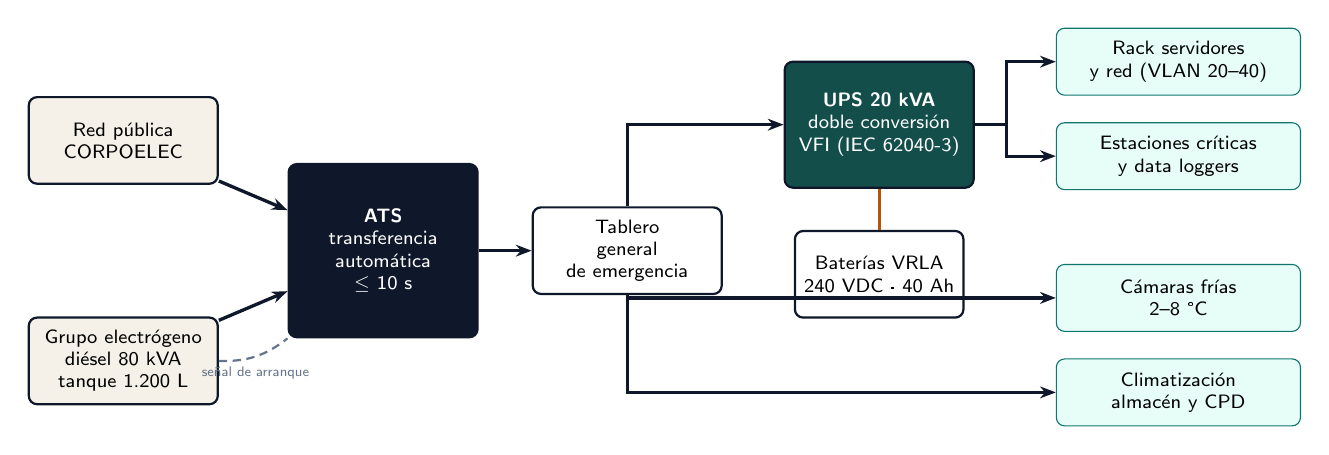
\begin{tikzpicture}[
  font=\sffamily\scriptsize,
  caja/.style={draw=fvTinta,fill=white,rounded corners=3pt,thick,minimum width=2.4cm,minimum height=1.1cm,align=center},
  carga/.style={draw=fvVerde,fill=fvVerdeClaro!50,rounded corners=3pt,minimum width=3.1cm,minimum height=0.85cm,align=center},
  linea/.style={-{Stealth[length=2mm]},very thick,draw=fvTinta},
]
  \node[caja,fill=fvArena] (red) at (0,1.4) {Red pública\\CORPOELEC};
  \node[caja,fill=fvArena] (gen) at (0,-1.4) {Grupo electrógeno\\diésel 80~kVA\\tanque 1.200~L};
  \node[caja,fill=fvTinta,text=white,minimum height=2.2cm] (ats) at (3.3,0) {\textbf{ATS}\\transferencia\\automática\\$\leq$ 10~s};
  \node[caja] (tg) at (6.4,0) {Tablero\\general\\de emergencia};
  \node[caja,fill=fvVerdeOsc,text=white,minimum height=1.6cm] (ups) at (9.6,1.6) {\textbf{UPS 20~kVA}\\doble conversión\\VFI (IEC 62040-3)};
  \node[caja,minimum width=1.9cm] (bat) at (9.6,-0.3) {Baterías VRLA\\240~VDC · 40~Ah};
  \node[carga] (c1) at (13.4,2.4) {Rack servidores\\y red (VLAN 20--40)};
  \node[carga] (c2) at (13.4,1.2) {Estaciones críticas\\y data loggers};
  \node[carga] (c3) at (13.4,-0.6) {Cámaras frías\\2--8~°C};
  \node[carga] (c4) at (13.4,-1.8) {Climatización\\almacén y CPD};

  \draw[linea] (red) -- (ats);
  \draw[linea] (gen) -- (ats);
  \draw[linea] (ats) -- (tg);
  \draw[linea] (tg.north) |- (ups.west);
  \draw[linea] (ups.east) -- ++(0.4,0) |- (c1.west);
  \draw[linea] (ups.east) -- ++(0.4,0) |- (c2.west);
  \draw[very thick,draw=fvAmbar] (ups.south) -- (bat.north);
  \draw[linea] (tg.south) |- (c3.west);
  \draw[linea] (tg.south) |- (c4.west);
  \draw[densely dashed,fvGris,thick] (gen.east) to[bend right=20] node[below,font=\sffamily\tiny]{señal de arranque} (ats.south west);
\end{tikzpicture}}
\caption{Cadena de suministro: red/generador $\rightarrow$ ATS $\rightarrow$ UPS de doble conversión $\rightarrow$ cargas críticas.}
\label{fig:electrica}
\end{figure}

El UPS de \textbf{doble conversión en línea} rectifica permanentemente la entrada y
regenera una onda senoidal limpia: las cargas críticas nunca ven el corte ni el tiempo de
transferencia del ATS (transferencia \SI{0}{\milli\second}). El grupo electrógeno alimenta
directamente las cargas de refrigeración, que toleran los segundos de transferencia gracias
a su inercia térmica.

\section{Cálculo del UPS}

\begin{table}[htbp]
\centering\small
\caption{Cargas críticas respaldadas por el UPS.}
\label{tab:cargas-ups}
\rowcolors{2}{fvArena}{white}
\begin{tabularx}{\textwidth}{@{}X r@{}}
\toprule
\rowcolor{fvVerdeOsc}\textcolor{white}{\textbf{Carga}} & \textcolor{white}{\textbf{Potencia (kW)}} \\
\midrule
Rack de servidores (firewall, aplicaciones, base de datos, almacenamiento) & 3,2 \\
Electrónica de red (core, acceso, puntos de acceso)                       & 0,8 \\
Estaciones críticas (24 equipos $\times$ \SI{150}{\watt})                  & 3,6 \\
Monitorización de cadena de frío (data loggers, controladores, BMS)        & 0,4 \\
Seguridad física (CCTV, control de acceso, iluminación de emergencia)       & 1,0 \\
\midrule
\textbf{Total $P_{\text{UPS}}$} & \textbf{9,0} \\
\bottomrule
\end{tabularx}
\end{table}

\paragraph{Potencia aparente.} Con factor de potencia de salida $FP=0{,}9$, un crecimiento
previsto del \SI{25}{\percent} y una carga máxima recomendada del \SI{80}{\percent}:
\[
S = \frac{P}{FP}\cdot\frac{1{,}25}{0{,}80}
  = \frac{9{,}0}{0{,}9}\cdot 1{,}5625 \approx \SI{15,6}{\kilo\voltampere}
  \;\Rightarrow\; \textbf{UPS comercial de } \SI{20}{\kilo\voltampere}.
\]

\paragraph{Banco de baterías.} La autonomía objetivo es de \SI{30}{\minute}: cubre con
holgura el arranque del generador ($\leq$ \SI{10}{\second}) y permite una intervención
manual si el arranque automático falla. Con eficiencia del inversor $\eta=0{,}95$ y
profundidad de descarga $DoD=0{,}8$:
\[
E = \frac{P\cdot t}{\eta\cdot DoD}=\frac{9{,}0\cdot 0{,}5}{0{,}95\cdot 0{,}8}\approx \SI{5,92}{\kilo\watt\hour}
\qquad
C = \frac{E}{V_{DC}}=\frac{5\,920}{240}\approx \SI{24,7}{\ampere\hour}.
\]
Se selecciona una cadena de 20 bloques VRLA de \SI{12}{\volt}/\SI{40}{\ampere\hour}
(\SI{9,6}{\kilo\watt\hour} nominales). Energía útil:
$9{,}6\times0{,}8\times0{,}95\approx\SI{7,3}{\kilo\watt\hour}$, es decir
$\approx$\SI{48}{\minute} a plena carga ($\approx$\SI{41}{\minute} aplicando un factor de
Peukert de 0,85).

\section{Cálculo del grupo electrógeno}

\begin{table}[htbp]
\centering\small
\caption{Cargas alimentadas por el grupo electrógeno.}
\label{tab:cargas-gen}
\rowcolors{2}{fvArena}{white}
\begin{tabularx}{\textwidth}{@{}X r@{}}
\toprule
\rowcolor{fvVerdeOsc}\textcolor{white}{\textbf{Carga}} & \textcolor{white}{\textbf{Potencia (kW)}} \\
\midrule
Cámaras frías \SIrange{2}{8}{\celsius} (2 compresores $\times$ \SI{4,5}{\kilo\watt}) & 9,0 \\
Refrigeradores farmacéuticos de laboratorio (6 $\times$ \SI{0,4}{\kilo\watt})        & 2,4 \\
Climatización de la sala de servidores (CPD)                                         & 5,0 \\
Climatización del almacén general ($\leq$ \SI{25}{\celsius})                         & 12,0 \\
Iluminación esencial                                                                  & 3,0 \\
Entrada del UPS ($9{,}0/0{,}95$ + recarga de baterías $\approx$ \SI{1,5}{\kilo\watt}) & 11,0 \\
\midrule
\textbf{Total $P_{\text{GEN}}$} & \textbf{42,4} \\
\bottomrule
\end{tabularx}
\end{table}

\[
S_{\text{GEN}}=\frac{42{,}4}{0{,}8}\times1{,}25\approx\SI{66,3}{\kilo\voltampere}
\;\Rightarrow\;\textbf{grupo de } \SI{80}{\kilo\voltampere}\;(\SI{64}{\kilo\watt}\text{ prime}).
\]
La carga resultante ($42{,}4/64\approx\SI{66}{\percent}$) evita el funcionamiento por
debajo del \SI{30}{\percent} (\emph{wet stacking}) y deja margen para la corriente de
arranque de los compresores (arranque escalonado por el BMS).

\paragraph{Combustible para 72 horas.} Con un consumo específico de
\SI{0,27}{\liter\per\kilo\watt\hour}:
\begin{align*}
\text{Peor caso (100\,\% de carga continua):}\quad & 42{,}4\times0{,}27\times72\approx\SI{824}{\liter}\\
\text{Caso medio (ciclado de compresores, 75\,\%):}\quad & 31{,}8\times0{,}27\times72\approx\SI{618}{\liter}
\end{align*}
Se especifica un \textbf{tanque de \SI{1200}{\liter}}, que cubre el peor caso con una reserva
del \SI{46}{\percent} (más de \SI{100}{\hour} en el caso medio). El combustible se rota
semestralmente y se trata con biocida.

\section{Secuencia de transferencia automática (ATS)}

\begin{enumerate}
  \item \textbf{Corte de red} ($t=0$): el UPS pasa a baterías sin interrupción; las cámaras
  frías se apagan momentáneamente.
  \item \textbf{Confirmación} ($t=\SI{3}{\second}$): el ATS descarta microcortes y ordena el
  arranque del generador.
  \item \textbf{Transferencia} ($t\leq\SI{10}{\second}$): con tensión y frecuencia estables,
  el ATS conmuta al generador (NFPA~110 Nivel~1, Tipo~10).
  \item \textbf{Régimen de emergencia}: el BMS rearranca los compresores de forma escalonada
  y el UPS recarga baterías.
  \item \textbf{Retorno de red}: tras \SI{5}{\minute} de estabilidad se retransfiere y el
  generador funciona \SI{5}{\minute} en vacío para enfriarse.
\end{enumerate}

\begin{tecnico}[Preservación de la cadena de frío]
Las cámaras mantienen \SIrange{2}{8}{\celsius} entre 2 y 4 horas sin energía con las
puertas cerradas; la transferencia de segundos es irrelevante para el producto. Los
data loggers, respaldados por el UPS, registran cualquier excursión y Laboratorio la
refleja en el campo \cod{temperaturaRegistro} del lote: si el rango se superó, el sistema
impide aprobarlo y, por tanto, venderlo.
\end{tecnico}

\section{Pruebas y mantenimiento}
\begin{itemize}
  \item Prueba mensual del generador con carga (\SI{30}{\minute}, $\geq$\SI{50}{\percent}).
  \item Prueba trimestral de transferencia real del ATS en ventana de mantenimiento.
  \item Prueba anual de autonomía de baterías y sustitución preventiva cada 4--5 años.
  \item Registro de nivel de combustible en el BMS con alarma por debajo del \SI{60}{\percent}.
\end{itemize}

% =====================================================================
\chapter{Políticas de firewall}
% =====================================================================

\section{Principios}
\begin{itemize}
  \item Cadena \cod{forward} con \textbf{política por defecto DROP}: todo flujo entre
  segmentos debe estar permitido explícitamente.
  \item Inspección con estado: \cod{ct state established,related accept} como primera regla
  y descarte de paquetes \cod{invalid}.
  \item La regla de aislamiento de datos se evalúa \emph{antes} que las reglas permisivas de
  oficinas, de modo que ningún cambio posterior pueda abrirla por accidente.
\end{itemize}

\section{Matriz de reglas \emph{forward}}

\begin{table}[htbp]
\centering\small
\caption{Matriz de filtrado de \cod{fw-01} (orden de evaluación).}
\label{tab:fw-forward}
\rowcolors{2}{fvArena}{white}
\begin{tabularx}{\textwidth}{@{}c L{2.9cm} L{2.6cm} L{2.0cm} c X@{}}
\toprule
\rowcolor{fvVerdeOsc}
\textcolor{white}{\textbf{\#}} & \textcolor{white}{\textbf{Origen}} & \textcolor{white}{\textbf{Destino}} &
\textcolor{white}{\textbf{Protocolo}} & \textcolor{white}{\textbf{Acción}} & \textcolor{white}{\textbf{Justificación}} \\
\midrule
1 & Cualquiera & Cualquiera & estado est./rel. & \permitir & Retorno de sesiones autorizadas \\
2 & Cualquiera & Cualquiera & estado inválido & \denegar & Paquetes malformados o fuera de sesión \\
3 & Oficinas 210--240 & Datos 10.10.40.0/24 & todos (incl. ICMP) & \denegar & Anti-ransomware: datos invisibles para estaciones \\
4 & Oficinas 210--240 & DMZ y Apps & ICMP echo-request & \permitir & Diagnóstico de conectividad \\
5 & Oficinas 210--240 & DMZ 10.10.20.0/24 & todos & \permitir & Acceso a la intranet \\
6 & Oficinas 210--240 & Apps 10.10.30.0/24 & todos & \permitir & Servicios de aplicación \\
7 & Proxy 10.10.20.10 & API 10.10.30.20 & TCP/3000 & \permitir & Proxy inverso $\rightarrow$ NestJS \\
8 & Apps 10.10.30.0/24 & BD 10.10.40.10 & TCP/5432 & \permitir & Único acceso a PostgreSQL \\
9 & Cualquiera & Cualquiera & todos & \denegar & Política por defecto (contabilizada) \\
\bottomrule
\end{tabularx}
\end{table}

\section{Traducción de direcciones (NAT)}

\begin{table}[htbp]
\centering\small
\caption{Reglas \cod{postrouting} de la tabla \cod{ip nat}.}
\label{tab:fw-nat}
\rowcolors{2}{fvArena}{white}
\begin{tabularx}{\textwidth}{@{}L{3.2cm} L{2.6cm} l X@{}}
\toprule
\rowcolor{fvVerdeOsc}
\textcolor{white}{\textbf{Origen}} & \textcolor{white}{\textbf{Destino}} & \textcolor{white}{\textbf{Acción}} &
\textcolor{white}{\textbf{Propósito}} \\
\midrule
Oficinas 210--240 & cualquiera (\cod{eth*}) & masquerade & Retorno garantizado: los servidores responden a la IP .254 del firewall \\
DMZ 10.10.20.0/24 & Apps & masquerade & Enrutamiento simétrico del proxy hacia la API \\
Apps 10.10.30.0/24 & Datos & masquerade & La BD responde por \cod{fw-01} sin rutas estáticas \\
\bottomrule
\end{tabularx}
\end{table}

El \emph{masquerade} resuelve un problema propio de las redes Docker: cada servidor conserva
como puerta de enlace el puente del anfitrión (\cod{.1}); sin traducción, las respuestas
a las oficinas intentarían salir por ese puente y se perderían (enrutamiento asimétrico).
Al reescribir el origen con la IP del firewall en el segmento de destino, el retorno queda
anclado a \cod{fw-01}, que deshace la traducción gracias a \emph{conntrack}.

\section{Configuración nftables}

\begin{lstlisting}[language=nft,caption={Extracto de \cod{/etc/nftables.conf} en \cod{fw-01}.},label=lst:nft]
define OFICINAS = { 10.10.210.0/24, 10.10.220.0/24, 10.10.230.0/24, 10.10.240.0/24 }
define DMZ   = 10.10.20.0/24
define APPS  = 10.10.30.0/24
define DATOS = 10.10.40.0/24

table inet filtro {
  chain forward {
    type filter hook forward priority filter; policy drop;
    ct state established,related accept
    ct state invalid counter drop
    ip saddr $OFICINAS ip daddr $DATOS counter drop
    ip saddr $OFICINAS ip daddr { $DMZ, $APPS } icmp type echo-request counter accept
    ip saddr $OFICINAS ip daddr $DMZ  counter accept
    ip saddr $OFICINAS ip daddr $APPS counter accept
    ip saddr 10.10.20.10 ip daddr 10.10.30.20 tcp dport 3000 counter accept
    ip saddr $APPS ip daddr 10.10.40.10 tcp dport 5432 counter accept
    counter comment "Descartado por politica"
  }
}

table ip nat {
  chain postrouting {
    type nat hook postrouting priority srcnat; policy accept;
    ip saddr $OFICINAS oifname "eth*" masquerade
    ip saddr $DMZ  ip daddr $APPS  oifname "eth*" masquerade
    ip saddr $APPS ip daddr $DATOS oifname "eth*" masquerade
  }
}
\end{lstlisting}

\section{Verificación}

El script \cod{pruebas\_oficina.sh}, incluido en cada estación, comprueba la política:

\begin{lstlisting}[language=bash]
docker exec pc_ventas_01 pruebas_oficina.sh farmaceutico1 password_ventas_123
#  [OK]   Ping a DMZ (10.10.20.10)
#  [OK]   Ping a Apps (10.10.30.20)
#  [OK]   HTTP intranet.farmaceutica.local
#  [OK]   Ping a Datos bloqueado
#  [OK]   PostgreSQL 10.10.40.10:5432 inaccesible
#  [OK]   Login correcto. Rol: ventas

docker exec fw-01 nft list ruleset          # contadores por regla
\end{lstlisting}

% =====================================================================
\appendix
\chapter{Despliegue}
% =====================================================================

\begin{lstlisting}[language=bash]
unzip proyectoFarmaVita_SEG.INF-URU.zip && cd proyectoFarmaVita_SEG.INF-URU
docker compose up -d --build
docker compose ps
# Intranet web: http://localhost:8080  (o intranet.farmaceutica.local:8080)
# Terminal de almacén:
docker exec -it pc_almacen_01 terminal_almacen
\end{lstlisting}

\begin{table}[htbp]
\centering\small
\caption{Componentes del repositorio.}
\rowcolors{2}{fvArena}{white}
\begin{tabularx}{\textwidth}{@{}l X@{}}
\toprule
\rowcolor{fvVerdeOsc}\textcolor{white}{\textbf{Ruta}} & \textcolor{white}{\textbf{Contenido}} \\
\midrule
\cod{docker-compose.yml}, \cod{.env} & Orquestación de 9 servicios y 7 redes \\
\cod{firewall/}         & Imagen Alpine con nftables, \cod{nftables.conf} y \cod{entrypoint.sh} \\
\cod{nginx/}            & Proxy inverso (vhost \cod{intranet.farmaceutica.local}) y compilación del frontend \\
\cod{ldap/bootstrap/}   & LDIF de unidades organizativas, usuarios y grupos \\
\cod{db/init/}          & Endurecimiento de PostgreSQL y esquema de auditoría \\
\cod{backend/}          & API NestJS: Auth, Inventario, Laboratorio, Ventas \\
\cod{frontend/}         & SPA React + Vite + TypeScript \\
\cod{terminal\_almacen/} & Cliente TUI en Rust (ratatui + ureq), binario estático musl \\
\cod{oficina/}          & Imagen de estación de trabajo y script de pruebas \\
\cod{docs/}             & Este informe \\
\bottomrule
\end{tabularx}
\end{table}

\end{document}
